% Options for packages loaded elsewhere
\PassOptionsToPackage{unicode}{hyperref}
\PassOptionsToPackage{hyphens}{url}
\documentclass[
]{article}
\usepackage{xcolor}
\usepackage[margin=1in]{geometry}
\usepackage{amsmath,amssymb}
\setcounter{secnumdepth}{-\maxdimen} % remove section numbering
\usepackage{iftex}
\ifPDFTeX
  \usepackage[T1]{fontenc}
  \usepackage[utf8]{inputenc}
  \usepackage{textcomp} % provide euro and other symbols
\else % if luatex or xetex
  \usepackage{unicode-math} % this also loads fontspec
  \defaultfontfeatures{Scale=MatchLowercase}
  \defaultfontfeatures[\rmfamily]{Ligatures=TeX,Scale=1}
\fi
\usepackage{lmodern}
\ifPDFTeX\else
  % xetex/luatex font selection
\fi
% Use upquote if available, for straight quotes in verbatim environments
\IfFileExists{upquote.sty}{\usepackage{upquote}}{}
\IfFileExists{microtype.sty}{% use microtype if available
  \usepackage[]{microtype}
  \UseMicrotypeSet[protrusion]{basicmath} % disable protrusion for tt fonts
}{}
\makeatletter
\@ifundefined{KOMAClassName}{% if non-KOMA class
  \IfFileExists{parskip.sty}{%
    \usepackage{parskip}
  }{% else
    \setlength{\parindent}{0pt}
    \setlength{\parskip}{6pt plus 2pt minus 1pt}}
}{% if KOMA class
  \KOMAoptions{parskip=half}}
\makeatother
\usepackage{color}
\usepackage{fancyvrb}
\newcommand{\VerbBar}{|}
\newcommand{\VERB}{\Verb[commandchars=\\\{\}]}
\DefineVerbatimEnvironment{Highlighting}{Verbatim}{commandchars=\\\{\}}
% Add ',fontsize=\small' for more characters per line
\usepackage{framed}
\definecolor{shadecolor}{RGB}{248,248,248}
\newenvironment{Shaded}{\begin{snugshade}}{\end{snugshade}}
\newcommand{\AlertTok}[1]{\textcolor[rgb]{0.94,0.16,0.16}{#1}}
\newcommand{\AnnotationTok}[1]{\textcolor[rgb]{0.56,0.35,0.01}{\textbf{\textit{#1}}}}
\newcommand{\AttributeTok}[1]{\textcolor[rgb]{0.13,0.29,0.53}{#1}}
\newcommand{\BaseNTok}[1]{\textcolor[rgb]{0.00,0.00,0.81}{#1}}
\newcommand{\BuiltInTok}[1]{#1}
\newcommand{\CharTok}[1]{\textcolor[rgb]{0.31,0.60,0.02}{#1}}
\newcommand{\CommentTok}[1]{\textcolor[rgb]{0.56,0.35,0.01}{\textit{#1}}}
\newcommand{\CommentVarTok}[1]{\textcolor[rgb]{0.56,0.35,0.01}{\textbf{\textit{#1}}}}
\newcommand{\ConstantTok}[1]{\textcolor[rgb]{0.56,0.35,0.01}{#1}}
\newcommand{\ControlFlowTok}[1]{\textcolor[rgb]{0.13,0.29,0.53}{\textbf{#1}}}
\newcommand{\DataTypeTok}[1]{\textcolor[rgb]{0.13,0.29,0.53}{#1}}
\newcommand{\DecValTok}[1]{\textcolor[rgb]{0.00,0.00,0.81}{#1}}
\newcommand{\DocumentationTok}[1]{\textcolor[rgb]{0.56,0.35,0.01}{\textbf{\textit{#1}}}}
\newcommand{\ErrorTok}[1]{\textcolor[rgb]{0.64,0.00,0.00}{\textbf{#1}}}
\newcommand{\ExtensionTok}[1]{#1}
\newcommand{\FloatTok}[1]{\textcolor[rgb]{0.00,0.00,0.81}{#1}}
\newcommand{\FunctionTok}[1]{\textcolor[rgb]{0.13,0.29,0.53}{\textbf{#1}}}
\newcommand{\ImportTok}[1]{#1}
\newcommand{\InformationTok}[1]{\textcolor[rgb]{0.56,0.35,0.01}{\textbf{\textit{#1}}}}
\newcommand{\KeywordTok}[1]{\textcolor[rgb]{0.13,0.29,0.53}{\textbf{#1}}}
\newcommand{\NormalTok}[1]{#1}
\newcommand{\OperatorTok}[1]{\textcolor[rgb]{0.81,0.36,0.00}{\textbf{#1}}}
\newcommand{\OtherTok}[1]{\textcolor[rgb]{0.56,0.35,0.01}{#1}}
\newcommand{\PreprocessorTok}[1]{\textcolor[rgb]{0.56,0.35,0.01}{\textit{#1}}}
\newcommand{\RegionMarkerTok}[1]{#1}
\newcommand{\SpecialCharTok}[1]{\textcolor[rgb]{0.81,0.36,0.00}{\textbf{#1}}}
\newcommand{\SpecialStringTok}[1]{\textcolor[rgb]{0.31,0.60,0.02}{#1}}
\newcommand{\StringTok}[1]{\textcolor[rgb]{0.31,0.60,0.02}{#1}}
\newcommand{\VariableTok}[1]{\textcolor[rgb]{0.00,0.00,0.00}{#1}}
\newcommand{\VerbatimStringTok}[1]{\textcolor[rgb]{0.31,0.60,0.02}{#1}}
\newcommand{\WarningTok}[1]{\textcolor[rgb]{0.56,0.35,0.01}{\textbf{\textit{#1}}}}
\usepackage{graphicx}
\makeatletter
\newsavebox\pandoc@box
\newcommand*\pandocbounded[1]{% scales image to fit in text height/width
  \sbox\pandoc@box{#1}%
  \Gscale@div\@tempa{\textheight}{\dimexpr\ht\pandoc@box+\dp\pandoc@box\relax}%
  \Gscale@div\@tempb{\linewidth}{\wd\pandoc@box}%
  \ifdim\@tempb\p@<\@tempa\p@\let\@tempa\@tempb\fi% select the smaller of both
  \ifdim\@tempa\p@<\p@\scalebox{\@tempa}{\usebox\pandoc@box}%
  \else\usebox{\pandoc@box}%
  \fi%
}
% Set default figure placement to htbp
\def\fps@figure{htbp}
\makeatother
\setlength{\emergencystretch}{3em} % prevent overfull lines
\providecommand{\tightlist}{%
  \setlength{\itemsep}{0pt}\setlength{\parskip}{0pt}}
\usepackage{bookmark}
\IfFileExists{xurl.sty}{\usepackage{xurl}}{} % add URL line breaks if available
\urlstyle{same}
% fallback for those not using the hyperref driver hyperxmp:
\makeatletter
\@ifundefined{xmpquote}{\newcommand{\xmpquote}[1]{#1}}{}
\makeatother
\hypersetup{
  pdftitle={Golden\_Kelly\_Final\_Submission},
  pdfauthor={Kelly Golden},
  hidelinks,
  pdfcreator={LaTeX via pandoc}}

\title{Golden\_Kelly\_Final\_Submission}
\author{Kelly Golden}
\date{2026-11-11}

\begin{document}
\maketitle

Resources Used: Claude (Anthropic) was used in this assignment as noted
in the code comments throughout. It was also used to help select genes
of personal interest, draft the gene rationale and variable
descriptions, improve organization, and debug code errors.

Variables Chosen: My primary gene is \emph{CXCR2}, a receptor on
neutrophils that responds to the inflammatory signal IL-8. Inflammation
is thought to play a role in preeclampsia, which made \emph{CXCR2} an
interesting gene to explore. My continuous covariate is maternal vitamin
D (mat\_vitD), measured as 25-hydroxyvitamin D in ng/mL at baseline. My
two categorical covariates are pregnancy outcome (preg\_preeclampsia:
normal vs.~preeclampsia) and obesity status, which I derived from
maternal BMI (mat\_BMI) using the WHO cut point of 30 kg/m² or higher.

Additional genes: I added \emph{NR0B2} and \emph{TRIB1} to contrast with
\emph{CXCR2}. \emph{NR0B2} is a nuclear receptor, expressed mainly in
the liver, that helps regulate bile acid, cholesterol, and glucose
metabolism; variants in it have been linked to obesity and early-onset
type 2 diabetes. \emph{TRIB1} controls fat production in the liver and
is also active in immune cells, so it bridges the other two; large
genetic studies have tied it to blood lipid levels and fatty liver
disease. Both connect to my broader interest in PFAS, which disrupt
nuclear-receptor signaling and are consistently associated with higher
cholesterol. Comparing the three lets me see whether the vitamin D and
obesity patterns seen for \emph{CXCR2} also appear in metabolic genes.

Heatmap and forest plot: For the heatmap, I selected seven more genes
related to inflammation (\emph{LYN}, \emph{PRKCD}, \emph{AQP9},
\emph{FOSL2}) and lipid metabolism (\emph{ACSL4}, \emph{EPHX2},
\emph{PEX12}), choosing ones that varied enough across participants to
visualize. For my additional plot, I used a forest plot to test whether
obesity explains the association between vitamin D and expression of
these ten genes.

\subsection{Load the data}\label{load-the-data}

\begin{Shaded}
\begin{Highlighting}[]
\CommentTok{\# read\_csv() automatically strips the invisible character (BOM) at the start}
\CommentTok{\# of the covariate file, so the first column is named "subjectID" correctly.}
\NormalTok{covar }\OtherTok{\textless{}{-}} \FunctionTok{read\_csv}\NormalTok{(}\StringTok{"/Users/kellygolden/Library/CloudStorage/OneDrive{-}DartmouthCollege/HSE 103/Final Project/Check in 1/GSE85307\_covar.csv"}\NormalTok{, }\AttributeTok{show\_col\_types =} \ConstantTok{FALSE}\NormalTok{, }\AttributeTok{name\_repair =} \StringTok{"unique\_quiet"}\NormalTok{)}

\CommentTok{\# gene expression: rows = probe IDs, columns = samples (GEO IDs).}
\CommentTok{\# the first column has no name in the file, so rename it PROBEID.}
\NormalTok{geneExp }\OtherTok{\textless{}{-}} \FunctionTok{read\_csv}\NormalTok{(}\StringTok{"/Users/kellygolden/Library/CloudStorage/OneDrive{-}DartmouthCollege/HSE 103/Final Project/Check in 1/GSE85307\_geneExpression.csv"}\NormalTok{, }\AttributeTok{show\_col\_types =} \ConstantTok{FALSE}\NormalTok{,}\AttributeTok{name\_repair =} \StringTok{"unique\_quiet"}\NormalTok{) }\SpecialCharTok{\%\textgreater{}\%}
  \FunctionTok{rename}\NormalTok{(}\AttributeTok{PROBEID =} \DecValTok{1}\NormalTok{)}

\CommentTok{\# linker file: probe ID {-}\textgreater{} gene name}
\NormalTok{geneNames }\OtherTok{\textless{}{-}} \FunctionTok{read\_csv}\NormalTok{(}\StringTok{"/Users/kellygolden/Library/CloudStorage/OneDrive{-}DartmouthCollege/HSE 103/Final Project/Check in 1/GSE85307\_geneNames.csv"}\NormalTok{, }\AttributeTok{show\_col\_types =} \ConstantTok{FALSE}\NormalTok{, }\AttributeTok{name\_repair =} \StringTok{"unique\_quiet"}\NormalTok{)}

\FunctionTok{dim}\NormalTok{(covar)}
\end{Highlighting}
\end{Shaded}

\begin{verbatim}
## [1] 157  10
\end{verbatim}

\begin{Shaded}
\begin{Highlighting}[]
\FunctionTok{dim}\NormalTok{(geneExp)   }
\end{Highlighting}
\end{Shaded}

\begin{verbatim}
## [1] 500 158
\end{verbatim}

\subsection{Clean the covariates}\label{clean-the-covariates}

Each covariate value (except the IDs) has a text label in front of it,
like \texttt{"age\_years:\ 31...."} or
\texttt{"pregnancy\_condition:\ Normal"}. I have to remove everything up
to and including the \texttt{":\ "} and then convert to the right type
of variable.

\begin{Shaded}
\begin{Highlighting}[]
\CommentTok{\# Look at the raw format first}
\FunctionTok{head}\NormalTok{(covar}\SpecialCharTok{$}\NormalTok{mat\_age\_yrs, }\DecValTok{3}\NormalTok{)}
\end{Highlighting}
\end{Shaded}

\begin{verbatim}
## [1] "age_years: 31.06639288" "age_years: 27.79466119" "age_years: 34.31895962"
\end{verbatim}

\begin{Shaded}
\begin{Highlighting}[]
\CommentTok{\# columns 3 to 10 have the "label: value"}
\ControlFlowTok{for}\NormalTok{ (col }\ControlFlowTok{in} \FunctionTok{names}\NormalTok{(covar)[}\DecValTok{3}\SpecialCharTok{:}\DecValTok{10}\NormalTok{]) \{}
\NormalTok{  covar[[col]] }\OtherTok{\textless{}{-}} \FunctionTok{sub}\NormalTok{(}\StringTok{".*: "}\NormalTok{, }\StringTok{""}\NormalTok{, covar[[col]])   }\CommentTok{\# keep only the part after ":"}
\NormalTok{\} }\CommentTok{\# Claude helped with this cleaning code}

\CommentTok{\# convert from text to numbers}
\NormalTok{numVars }\OtherTok{\textless{}{-}} \FunctionTok{c}\NormalTok{(}\StringTok{"mat\_age\_yrs"}\NormalTok{, }\StringTok{"delivery\_gestAge\_wks"}\NormalTok{,}
             \StringTok{"sampleCollection\_gestAge\_wks"}\NormalTok{, }\StringTok{"mat\_BMI"}\NormalTok{, }\StringTok{"mat\_vitD"}\NormalTok{)}
\ControlFlowTok{for}\NormalTok{ (col }\ControlFlowTok{in}\NormalTok{ numVars) \{}
\NormalTok{  covar[[col]] }\OtherTok{\textless{}{-}} \FunctionTok{as.numeric}\NormalTok{(covar[[col]])}
\NormalTok{\}}

\CommentTok{\# convert categorical variables to factors with clear labels (Claude helped here)}
\NormalTok{covar}\SpecialCharTok{$}\NormalTok{preg\_preeclampsia }\OtherTok{\textless{}{-}} \FunctionTok{factor}\NormalTok{(covar}\SpecialCharTok{$}\NormalTok{preg\_preeclampsia,}
                                  \AttributeTok{levels =} \FunctionTok{c}\NormalTok{(}\StringTok{"Normal"}\NormalTok{, }\StringTok{"Preeclampsia"}\NormalTok{))}
\NormalTok{covar}\SpecialCharTok{$}\NormalTok{mat\_asthma }\OtherTok{\textless{}{-}} \FunctionTok{factor}\NormalTok{(covar}\SpecialCharTok{$}\NormalTok{mat\_asthma, }\AttributeTok{levels =} \FunctionTok{c}\NormalTok{(}\DecValTok{0}\NormalTok{, }\DecValTok{1}\NormalTok{),}
                           \AttributeTok{labels =} \FunctionTok{c}\NormalTok{(}\StringTok{"Healthy"}\NormalTok{, }\StringTok{"Asthma"}\NormalTok{))}
\NormalTok{covar}\SpecialCharTok{$}\NormalTok{batch\_Microarray }\OtherTok{\textless{}{-}} \FunctionTok{factor}\NormalTok{(covar}\SpecialCharTok{$}\NormalTok{batch\_Microarray)}

\CommentTok{\# derived categorical variable: obesity status from BMI (WHO: BMI \textgreater{}= 30)}
\NormalTok{covar}\SpecialCharTok{$}\NormalTok{obesity }\OtherTok{\textless{}{-}} \FunctionTok{factor}\NormalTok{(}\FunctionTok{ifelse}\NormalTok{(covar}\SpecialCharTok{$}\NormalTok{mat\_BMI }\SpecialCharTok{\textgreater{}=} \DecValTok{30}\NormalTok{, }\StringTok{"Obese"}\NormalTok{, }\StringTok{"Not obese"}\NormalTok{),}
                        \AttributeTok{levels =} \FunctionTok{c}\NormalTok{(}\StringTok{"Not obese"}\NormalTok{, }\StringTok{"Obese"}\NormalTok{))}

\CommentTok{\# confirm no missing values were created by the conversions (Claude helped here)}
\FunctionTok{colSums}\NormalTok{(}\FunctionTok{is.na}\NormalTok{(covar))}
\end{Highlighting}
\end{Shaded}

\begin{verbatim}
##                    subjectID                        geoID 
##                            0                            0 
##                  mat_age_yrs            preg_preeclampsia 
##                            0                            0 
##         delivery_gestAge_wks sampleCollection_gestAge_wks 
##                            0                            0 
##             batch_Microarray                      mat_BMI 
##                            0                            0 
##                     mat_vitD                   mat_asthma 
##                            0                            0 
##                      obesity 
##                            0
\end{verbatim}

\begin{Shaded}
\begin{Highlighting}[]
\FunctionTok{summary}\NormalTok{(covar[, }\FunctionTok{c}\NormalTok{(numVars, }\StringTok{"preg\_preeclampsia"}\NormalTok{, }\StringTok{"obesity"}\NormalTok{)])}
\end{Highlighting}
\end{Shaded}

\begin{verbatim}
##   mat_age_yrs    delivery_gestAge_wks sampleCollection_gestAge_wks
##  Min.   :18.43   Min.   :26.43        Min.   :10.00               
##  1st Qu.:22.15   1st Qu.:38.14        1st Qu.:12.14               
##  Median :26.57   Median :39.29        Median :13.43               
##  Mean   :26.38   Mean   :38.82        Mean   :14.13               
##  3rd Qu.:30.14   3rd Qu.:40.00        3rd Qu.:16.43               
##  Max.   :38.76   Max.   :42.00        Max.   :18.86               
##     mat_BMI         mat_vitD        preg_preeclampsia      obesity   
##  Min.   :17.95   Min.   : 5.11   Normal      :110     Not obese:100  
##  1st Qu.:22.90   1st Qu.:13.40   Preeclampsia: 47     Obese    : 57  
##  Median :27.33   Median :20.40                                       
##  Mean   :28.94   Mean   :22.98                                       
##  3rd Qu.:33.27   3rd Qu.:29.50                                       
##  Max.   :61.95   Max.   :80.80
\end{verbatim}

\subsection{Match the probes to the gene
names}\label{match-the-probes-to-the-gene-names}

\begin{Shaded}
\begin{Highlighting}[]
\CommentTok{\# Claude helped me choose which functions to apply for this section given}
\CommentTok{\# my R language is still developing}

\CommentTok{\# confirm every probe in the expression data has a gene name in the linker file}
\FunctionTok{all}\NormalTok{(geneExp}\SpecialCharTok{$}\NormalTok{PROBEID }\SpecialCharTok{\%in\%}\NormalTok{ geneNames}\SpecialCharTok{$}\NormalTok{PROBEID)   }\CommentTok{\# expect TRUE}
\end{Highlighting}
\end{Shaded}

\begin{verbatim}
## [1] TRUE
\end{verbatim}

\begin{Shaded}
\begin{Highlighting}[]
\NormalTok{geneExp }\OtherTok{\textless{}{-}}\NormalTok{ geneExp }\SpecialCharTok{\%\textgreater{}\%}
  \FunctionTok{left\_join}\NormalTok{(geneNames, }\AttributeTok{by =} \StringTok{"PROBEID"}\NormalTok{) }\SpecialCharTok{\%\textgreater{}\%}   \CommentTok{\# add a GENE column}
  \FunctionTok{relocate}\NormalTok{(GENE, }\AttributeTok{.after =}\NormalTok{ PROBEID)           }\CommentTok{\# move it next to PROBEID}

\CommentTok{\# count duplicated gene names (each gene should be one probe)}
\FunctionTok{sum}\NormalTok{(}\FunctionTok{duplicated}\NormalTok{(geneExp}\SpecialCharTok{$}\NormalTok{GENE))   }\CommentTok{\# expect 0}
\end{Highlighting}
\end{Shaded}

\begin{verbatim}
## [1] 0
\end{verbatim}

\subsection{Merge}\label{merge}

The expression data has samples as columns, while the covariates have
samples as rows. I reshaped the expression data to long format (one row
per gene per sample) and joined \emph{CXCR2} to the covariates to verify
the merge.

\begin{Shaded}
\begin{Highlighting}[]
\NormalTok{gene }\OtherTok{\textless{}{-}} \StringTok{"CXCR2"}

\NormalTok{geneLong }\OtherTok{\textless{}{-}}\NormalTok{ geneExp }\SpecialCharTok{\%\textgreater{}\%}
  \FunctionTok{select}\NormalTok{(}\SpecialCharTok{{-}}\NormalTok{PROBEID) }\SpecialCharTok{\%\textgreater{}\%}
  \FunctionTok{pivot\_longer}\NormalTok{(}\AttributeTok{cols =} \SpecialCharTok{{-}}\NormalTok{GENE, }\AttributeTok{names\_to =} \StringTok{"geoID"}\NormalTok{, }\AttributeTok{values\_to =} \StringTok{"expression"}\NormalTok{)}

\NormalTok{dat }\OtherTok{\textless{}{-}}\NormalTok{ geneLong }\SpecialCharTok{\%\textgreater{}\%}
  \FunctionTok{filter}\NormalTok{(GENE }\SpecialCharTok{==}\NormalTok{ gene) }\SpecialCharTok{\%\textgreater{}\%}
  \FunctionTok{inner\_join}\NormalTok{(covar, }\AttributeTok{by =} \StringTok{"geoID"}\NormalTok{)}
\end{Highlighting}
\end{Shaded}

\subsection{Verify}\label{verify}

\begin{Shaded}
\begin{Highlighting}[]
\CommentTok{\# Claude helped with the code below:}
\CommentTok{\# confirm the same samples are in both files}
\FunctionTok{setequal}\NormalTok{(covar}\SpecialCharTok{$}\NormalTok{geoID, }\FunctionTok{unique}\NormalTok{(geneLong}\SpecialCharTok{$}\NormalTok{geoID))   }\CommentTok{\# expect TRUE}
\end{Highlighting}
\end{Shaded}

\begin{verbatim}
## [1] TRUE
\end{verbatim}

\begin{Shaded}
\begin{Highlighting}[]
\CommentTok{\# confirm no one was lost or duplicated in the join}
\FunctionTok{nrow}\NormalTok{(dat)                        }\CommentTok{\# expect 157}
\end{Highlighting}
\end{Shaded}

\begin{verbatim}
## [1] 157
\end{verbatim}

\begin{Shaded}
\begin{Highlighting}[]
\FunctionTok{sum}\NormalTok{(}\FunctionTok{duplicated}\NormalTok{(dat}\SpecialCharTok{$}\NormalTok{geoID))       }\CommentTok{\# expect 0}
\end{Highlighting}
\end{Shaded}

\begin{verbatim}
## [1] 0
\end{verbatim}

\begin{Shaded}
\begin{Highlighting}[]
\CommentTok{\# the joined value should match the raw value}
\NormalTok{check\_id }\OtherTok{\textless{}{-}}\NormalTok{ dat}\SpecialCharTok{$}\NormalTok{geoID[}\DecValTok{1}\NormalTok{]}
\NormalTok{raw\_value }\OtherTok{\textless{}{-}}\NormalTok{ geneExp }\SpecialCharTok{\%\textgreater{}\%} \FunctionTok{filter}\NormalTok{(GENE }\SpecialCharTok{==}\NormalTok{ gene) }\SpecialCharTok{\%\textgreater{}\%} \FunctionTok{pull}\NormalTok{(}\FunctionTok{all\_of}\NormalTok{(check\_id))}
\NormalTok{dat}\SpecialCharTok{$}\NormalTok{expression[}\DecValTok{1}\NormalTok{] }\SpecialCharTok{==}\NormalTok{ raw\_value   }\CommentTok{\# expect TRUE}
\end{Highlighting}
\end{Shaded}

\begin{verbatim}
## [1] TRUE
\end{verbatim}

\subsection{Plot theme}\label{plot-theme}

\begin{Shaded}
\begin{Highlighting}[]
\NormalTok{theme\_pub }\OtherTok{\textless{}{-}} \FunctionTok{theme\_classic}\NormalTok{(}\AttributeTok{base\_size =} \DecValTok{12}\NormalTok{) }\SpecialCharTok{+}
  \FunctionTok{theme}\NormalTok{(}\AttributeTok{axis.title   =} \FunctionTok{element\_text}\NormalTok{(}\AttributeTok{face =} \StringTok{"bold"}\NormalTok{),}
        \AttributeTok{axis.text    =} \FunctionTok{element\_text}\NormalTok{(}\AttributeTok{color =} \StringTok{"\#280003"}\NormalTok{),}
        \AttributeTok{legend.title =} \FunctionTok{element\_text}\NormalTok{(}\AttributeTok{face =} \StringTok{"bold"}\NormalTok{),}
        \AttributeTok{legend.position =} \StringTok{"top"}\NormalTok{)}

\NormalTok{obesityColors }\OtherTok{\textless{}{-}} \FunctionTok{c}\NormalTok{(}\StringTok{"Not obese"} \OtherTok{=} \StringTok{"\#4E8098"}\NormalTok{, }\StringTok{"Obese"} \OtherTok{=} \StringTok{"\#86BA90"}\NormalTok{)}
\end{Highlighting}
\end{Shaded}

\subsection{Combine all genes with
covariates}\label{combine-all-genes-with-covariates}

\begin{Shaded}
\begin{Highlighting}[]
\CommentTok{\# join all genes to the covariates so the function can pull out any gene}
\NormalTok{datAll }\OtherTok{\textless{}{-}}\NormalTok{ geneLong }\SpecialCharTok{\%\textgreater{}\%}
  \FunctionTok{inner\_join}\NormalTok{(covar, }\AttributeTok{by =} \StringTok{"geoID"}\NormalTok{)}

\FunctionTok{nrow}\NormalTok{(datAll)   }\CommentTok{\# expect 78500}
\end{Highlighting}
\end{Shaded}

\begin{verbatim}
## [1] 78500
\end{verbatim}

\subsection{Plotting function}\label{plotting-function}

\begin{Shaded}
\begin{Highlighting}[]
\NormalTok{plotGenes }\OtherTok{\textless{}{-}} \ControlFlowTok{function}\NormalTok{(dataAll, genes) \{}
  \ControlFlowTok{for}\NormalTok{ (g }\ControlFlowTok{in}\NormalTok{ genes) \{}
\NormalTok{    geneData }\OtherTok{\textless{}{-}}\NormalTok{ dataAll }\SpecialCharTok{\%\textgreater{}\%} \FunctionTok{filter}\NormalTok{(GENE }\SpecialCharTok{==}\NormalTok{ g)}

    \CommentTok{\# histogram}
\NormalTok{    histPlot }\OtherTok{\textless{}{-}} \FunctionTok{ggplot}\NormalTok{(geneData, }\FunctionTok{aes}\NormalTok{(}\AttributeTok{x =}\NormalTok{ expression)) }\SpecialCharTok{+}
      \FunctionTok{geom\_histogram}\NormalTok{(}\AttributeTok{bins =} \DecValTok{25}\NormalTok{, }\AttributeTok{fill =} \StringTok{"\#713E5A"}\NormalTok{, }\AttributeTok{color =} \StringTok{"white"}\NormalTok{) }\SpecialCharTok{+}
      \FunctionTok{labs}\NormalTok{(}\AttributeTok{x =} \FunctionTok{bquote}\NormalTok{(}\FunctionTok{bolditalic}\NormalTok{(.(g)) }\SpecialCharTok{\textasciitilde{}}
                        \FunctionTok{bold}\NormalTok{(}\StringTok{"expression (log2 normalized intensity)"}\NormalTok{)),}
           \AttributeTok{y =} \StringTok{"Number of participants"}\NormalTok{) }\SpecialCharTok{+}
      \FunctionTok{scale\_y\_continuous}\NormalTok{(}\AttributeTok{expand =} \FunctionTok{expansion}\NormalTok{(}\AttributeTok{mult =} \FunctionTok{c}\NormalTok{(}\DecValTok{0}\NormalTok{, }\FloatTok{0.05}\NormalTok{))) }\SpecialCharTok{+}  \CommentTok{\# bars sit on the axis}
\NormalTok{      theme\_pub}
    \FunctionTok{print}\NormalTok{(histPlot)}

    \CommentTok{\# scatterplot}
\NormalTok{    scatterPlot }\OtherTok{\textless{}{-}} \FunctionTok{ggplot}\NormalTok{(geneData, }\FunctionTok{aes}\NormalTok{(}\AttributeTok{x =}\NormalTok{ mat\_vitD, }\AttributeTok{y =}\NormalTok{ expression)) }\SpecialCharTok{+}
      \FunctionTok{geom\_point}\NormalTok{(}\AttributeTok{color =} \StringTok{"\#713E5A"}\NormalTok{, }\AttributeTok{alpha =} \FloatTok{0.7}\NormalTok{, }\AttributeTok{size =} \DecValTok{2}\NormalTok{) }\SpecialCharTok{+}
      \FunctionTok{geom\_smooth}\NormalTok{(}\AttributeTok{method =} \StringTok{"lm"}\NormalTok{, }\AttributeTok{se =} \ConstantTok{TRUE}\NormalTok{, }\AttributeTok{color =} \StringTok{"\#280003"}\NormalTok{, }\AttributeTok{linewidth =} \FloatTok{0.8}\NormalTok{) }\SpecialCharTok{+}
      \FunctionTok{labs}\NormalTok{(}\AttributeTok{x =} \StringTok{"Maternal 25{-}hydroxyvitamin D (ng/mL)"}\NormalTok{,}
           \AttributeTok{y =} \FunctionTok{bquote}\NormalTok{(}\FunctionTok{bolditalic}\NormalTok{(.(g)) }\SpecialCharTok{\textasciitilde{}} \FunctionTok{bold}\NormalTok{(}\StringTok{"expression (log2)"}\NormalTok{))) }\SpecialCharTok{+}
\NormalTok{      theme\_pub}
    \FunctionTok{print}\NormalTok{(scatterPlot)}

    \CommentTok{\# boxplot}
\NormalTok{    boxPlot }\OtherTok{\textless{}{-}} \FunctionTok{ggplot}\NormalTok{(geneData, }\FunctionTok{aes}\NormalTok{(}\AttributeTok{x =}\NormalTok{ preg\_preeclampsia, }\AttributeTok{y =}\NormalTok{ expression, }\AttributeTok{fill =}\NormalTok{ obesity)) }\SpecialCharTok{+}
      \FunctionTok{geom\_boxplot}\NormalTok{(}\AttributeTok{outlier.shape =} \ConstantTok{NA}\NormalTok{, }\AttributeTok{width =} \FloatTok{0.6}\NormalTok{,}
                   \AttributeTok{position =} \FunctionTok{position\_dodge}\NormalTok{(}\AttributeTok{width =} \FloatTok{0.7}\NormalTok{)) }\SpecialCharTok{+}
      \CommentTok{\# show the participants on top of the boxes (Claude assisted)}
      \FunctionTok{geom\_point}\NormalTok{(}\AttributeTok{position =} \FunctionTok{position\_jitterdodge}\NormalTok{(}\AttributeTok{jitter.width =} \FloatTok{0.15}\NormalTok{,}
                                                 \AttributeTok{dodge.width =} \FloatTok{0.7}\NormalTok{,}
                                                 \AttributeTok{seed =} \DecValTok{123}\NormalTok{),  }\CommentTok{\# added a seed}
                 \AttributeTok{size =} \FloatTok{1.2}\NormalTok{, }\AttributeTok{alpha =} \FloatTok{0.5}\NormalTok{, }\AttributeTok{show.legend =} \ConstantTok{FALSE}\NormalTok{) }\SpecialCharTok{+}
      \FunctionTok{scale\_fill\_manual}\NormalTok{(}\AttributeTok{values =}\NormalTok{ obesityColors, }\AttributeTok{name =} \StringTok{"Obesity status"}\NormalTok{) }\SpecialCharTok{+}
      \FunctionTok{labs}\NormalTok{(}\AttributeTok{x =} \StringTok{"Pregnancy outcome"}\NormalTok{, }\AttributeTok{y =} \FunctionTok{bquote}\NormalTok{(}\FunctionTok{bolditalic}\NormalTok{(.(g)) }\SpecialCharTok{\textasciitilde{}} \FunctionTok{bold}\NormalTok{(}\StringTok{"expression (log2)"}\NormalTok{))) }\SpecialCharTok{+}
\NormalTok{      theme\_pub}
    \FunctionTok{print}\NormalTok{(boxPlot)}

\NormalTok{  \}}
\NormalTok{\}    }
\end{Highlighting}
\end{Shaded}

\subsection{Figure caption}\label{figure-caption}

\begin{Shaded}
\begin{Highlighting}[]
\CommentTok{\# Claude helped figure this code out}
\CommentTok{\# genes to plot}
\NormalTok{myGenes }\OtherTok{\textless{}{-}} \FunctionTok{c}\NormalTok{(}\StringTok{"CXCR2"}\NormalTok{, }\StringTok{"NR0B2"}\NormalTok{, }\StringTok{"TRIB1"}\NormalTok{)}

\CommentTok{\# build one caption per plot, in the order the function prints them}
\NormalTok{plotCaps }\OtherTok{\textless{}{-}} \FunctionTok{c}\NormalTok{()   }\CommentTok{\# start with an empty list of captions}
\ControlFlowTok{for}\NormalTok{ (g }\ControlFlowTok{in}\NormalTok{ myGenes) \{}
\NormalTok{  plotCaps }\OtherTok{\textless{}{-}} \FunctionTok{c}\NormalTok{(plotCaps,}
    \FunctionTok{paste0}\NormalTok{(}\StringTok{"}\SpecialCharTok{\textbackslash{}\textbackslash{}}\StringTok{textbf\{Distribution of }\SpecialCharTok{\textbackslash{}\textbackslash{}}\StringTok{textit\{"}\NormalTok{, g, }\StringTok{"\} expression.\} "}\NormalTok{,}
         \StringTok{"Expression values from 157 pregnant participants are log2{-}transformed "}\NormalTok{,}
         \StringTok{"normalized intensities from the Affymetrix Human Gene 1.0 ST Array, "}\NormalTok{,}
         \StringTok{"measured in blood collected at 10{-}{-}19 weeks\textquotesingle{} gestation."}\NormalTok{),}
    \FunctionTok{paste0}\NormalTok{(}\StringTok{"}\SpecialCharTok{\textbackslash{}\textbackslash{}}\StringTok{textbf\{Maternal vitamin D vs. }\SpecialCharTok{\textbackslash{}\textbackslash{}}\StringTok{textit\{"}\NormalTok{, g, }\StringTok{"\} expression.\} Each "}\NormalTok{,}
          \StringTok{"point is one participant (n = 157). The black line is a linear "}\NormalTok{,}
          \StringTok{"regression fit, and the gray band is its 95}\SpecialCharTok{\textbackslash{}\textbackslash{}}\StringTok{\% confidence interval."}\NormalTok{),}
    \FunctionTok{paste0}\NormalTok{(}\StringTok{"}\SpecialCharTok{\textbackslash{}\textbackslash{}}\StringTok{textbf\{}\SpecialCharTok{\textbackslash{}\textbackslash{}}\StringTok{textit\{"}\NormalTok{, g, }\StringTok{"\} expression by pregnancy outcome and obesity status.\} "}\NormalTok{,}
       \StringTok{"Obesity was defined as BMI $}\SpecialCharTok{\textbackslash{}\textbackslash{}}\StringTok{geq$ 30 kg/m². Boxes show the median and "}\NormalTok{,}
           \StringTok{"interquartile range, whiskers extend to 1.5 × IQR, and points are "}\NormalTok{,}
           \StringTok{"individual participants. Group sizes: Normal/not obese n = 79, "}\NormalTok{,  }
           \StringTok{"Normal/obese n = 31, Preeclampsia/not obese n = 21, Preeclampsia/obese "}\NormalTok{,}
           \StringTok{"n = 26."}\NormalTok{)}
\NormalTok{  )}
\NormalTok{\}}

\FunctionTok{length}\NormalTok{(plotCaps)   }\CommentTok{\# expect 9}
\end{Highlighting}
\end{Shaded}

\begin{verbatim}
## [1] 9
\end{verbatim}

\subsection{Box, Histogram, and
Scatterplots}\label{box-histogram-and-scatterplots}

\begin{Shaded}
\begin{Highlighting}[]
\CommentTok{\# run the function}
\FunctionTok{plotGenes}\NormalTok{(datAll, myGenes)}
\end{Highlighting}
\end{Shaded}

\begin{figure}
\centering
\pandocbounded{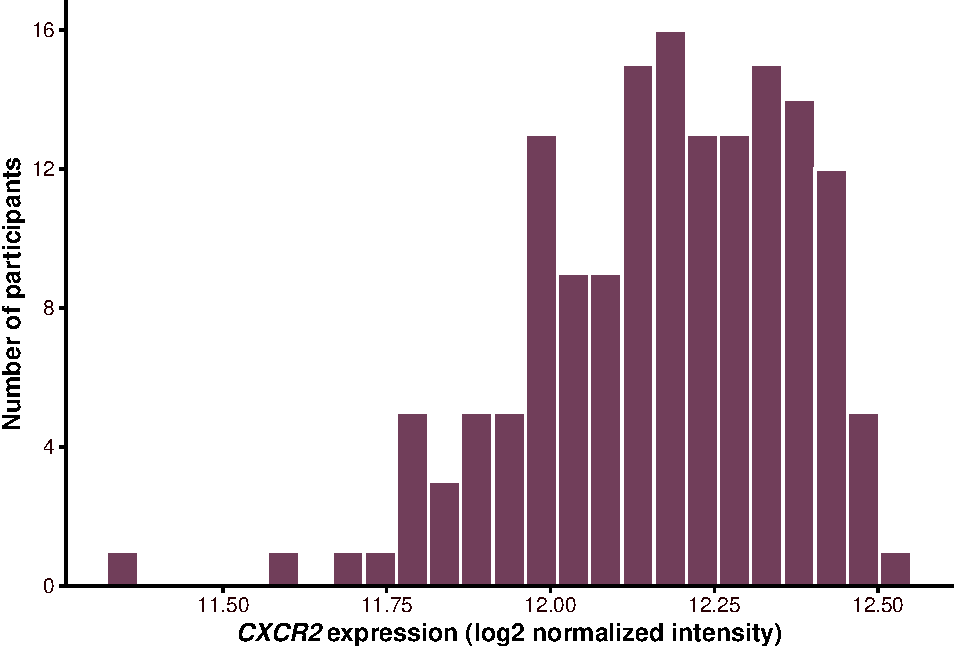
\includegraphics[keepaspectratio,alt={ Expression values from 157 pregnant participants are log2-transformed normalized intensities from the Affymetrix Human Gene 1.0 ST Array, measured in blood collected at 10--19 weeks' gestation.}]{Golden_Kelly_Final_Submission_files/figure-latex/plots-1.pdf}}
\caption{\textbf{Distribution of \textit{CXCR2} expression.} Expression
values from 157 pregnant participants are log2-transformed normalized
intensities from the Affymetrix Human Gene 1.0 ST Array, measured in
blood collected at 10--19 weeks' gestation.}
\end{figure}

\begin{figure}
\centering
\pandocbounded{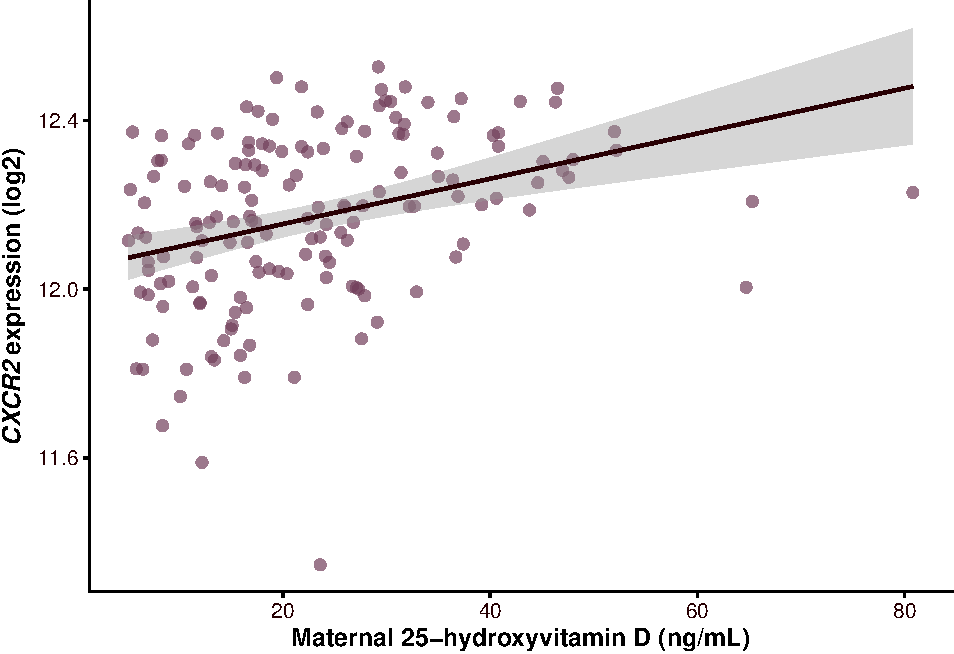
\includegraphics[keepaspectratio,alt={ Each point is one participant (n = 157). The black line is a linear regression fit, and the gray band is its 95\% confidence interval.}]{Golden_Kelly_Final_Submission_files/figure-latex/plots-2.pdf}}
\caption{\textbf{Maternal vitamin D vs. \textit{CXCR2} expression.} Each
point is one participant (n = 157). The black line is a linear
regression fit, and the gray band is its 95\% confidence interval.}
\end{figure}

\begin{figure}
\centering
\pandocbounded{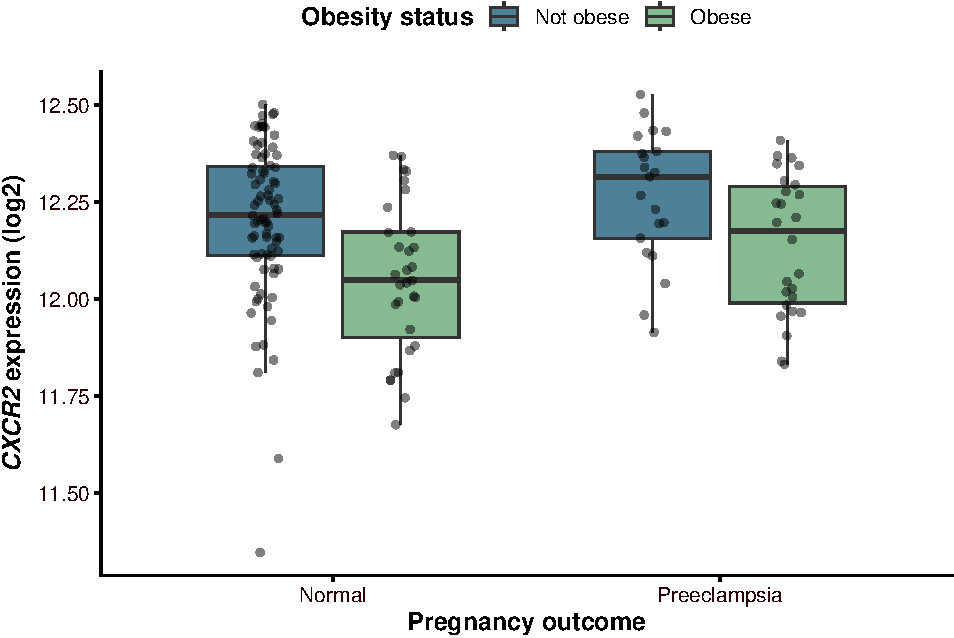
\includegraphics[keepaspectratio,alt={ Obesity was defined as BMI \textbackslash geq 30 kg/m². Boxes show the median and interquartile range, whiskers extend to 1.5 × IQR, and points are individual participants. Group sizes: Normal/not obese n = 79, Normal/obese n = 31, Preeclampsia/not obese n = 21, Preeclampsia/obese n = 26.}]{Golden_Kelly_Final_Submission_files/figure-latex/plots-3.pdf}}
\caption{\textbf{\textit{CXCR2} expression by pregnancy outcome and obesity status.}
Obesity was defined as BMI \(\geq\) 30 kg/m². Boxes show the median and
interquartile range, whiskers extend to 1.5 × IQR, and points are
individual participants. Group sizes: Normal/not obese n = 79,
Normal/obese n = 31, Preeclampsia/not obese n = 21, Preeclampsia/obese n
= 26.}
\end{figure}

\begin{figure}
\centering
\pandocbounded{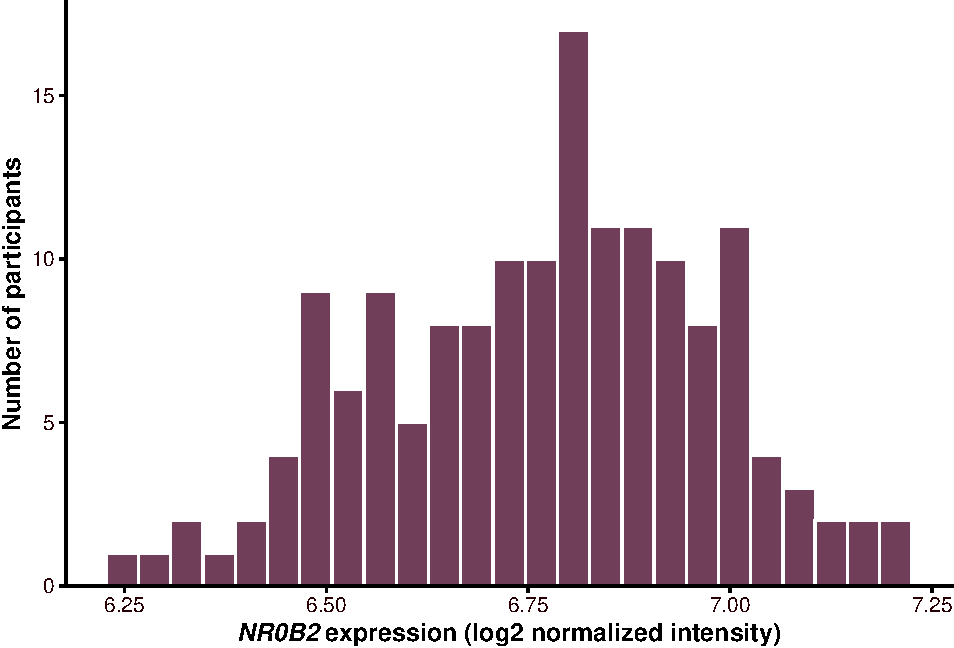
\includegraphics[keepaspectratio,alt={ Expression values from 157 pregnant participants are log2-transformed normalized intensities from the Affymetrix Human Gene 1.0 ST Array, measured in blood collected at 10--19 weeks' gestation.}]{Golden_Kelly_Final_Submission_files/figure-latex/plots-4.pdf}}
\caption{\textbf{Distribution of \textit{NR0B2} expression.} Expression
values from 157 pregnant participants are log2-transformed normalized
intensities from the Affymetrix Human Gene 1.0 ST Array, measured in
blood collected at 10--19 weeks' gestation.}
\end{figure}

\begin{figure}
\centering
\pandocbounded{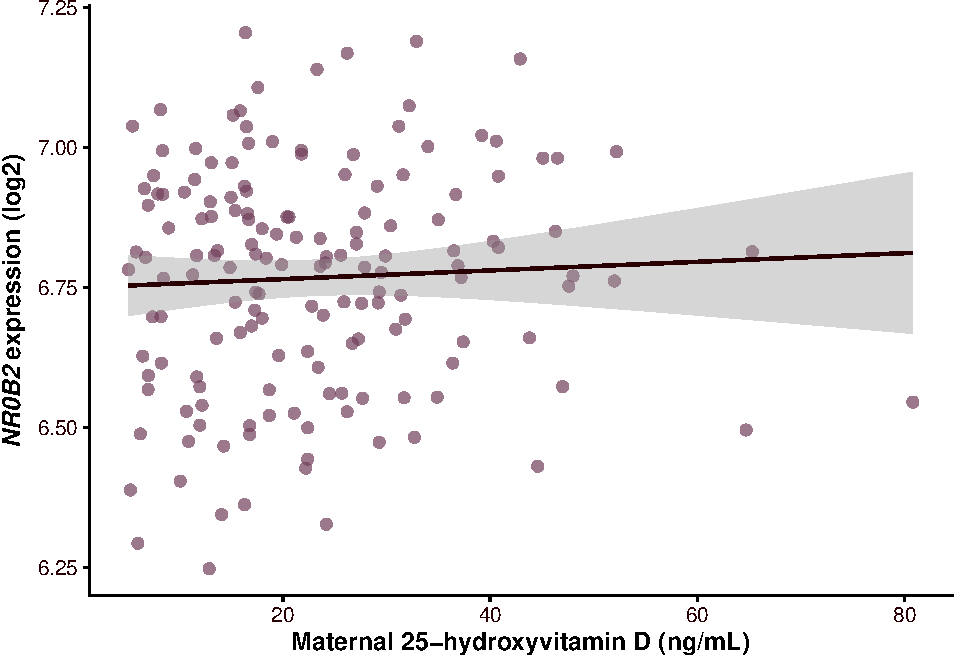
\includegraphics[keepaspectratio,alt={ Each point is one participant (n = 157). The black line is a linear regression fit, and the gray band is its 95\% confidence interval.}]{Golden_Kelly_Final_Submission_files/figure-latex/plots-5.pdf}}
\caption{\textbf{Maternal vitamin D vs. \textit{NR0B2} expression.} Each
point is one participant (n = 157). The black line is a linear
regression fit, and the gray band is its 95\% confidence interval.}
\end{figure}

\begin{figure}
\centering
\pandocbounded{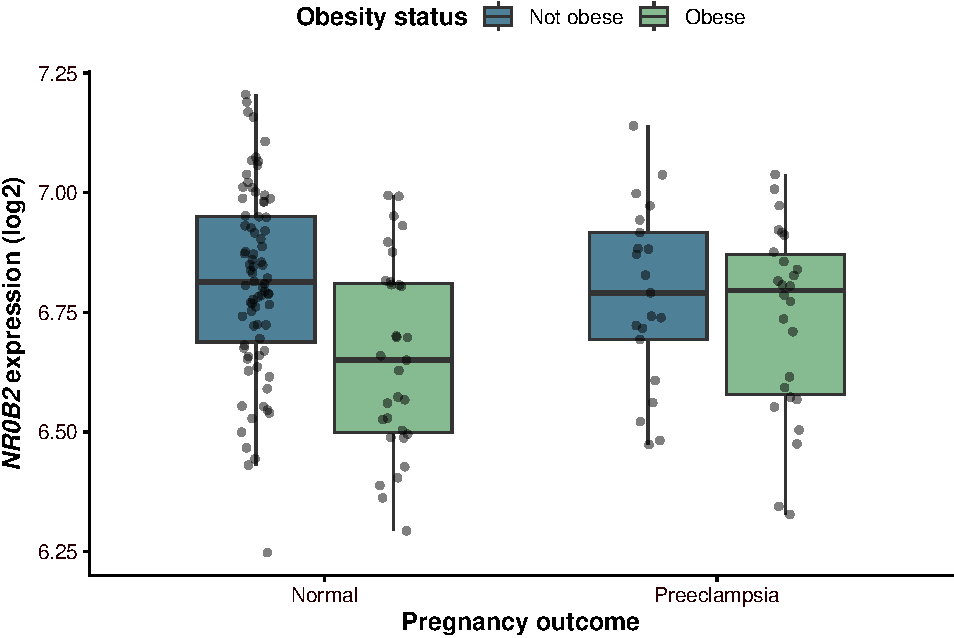
\includegraphics[keepaspectratio,alt={ Obesity was defined as BMI \textbackslash geq 30 kg/m². Boxes show the median and interquartile range, whiskers extend to 1.5 × IQR, and points are individual participants. Group sizes: Normal/not obese n = 79, Normal/obese n = 31, Preeclampsia/not obese n = 21, Preeclampsia/obese n = 26.}]{Golden_Kelly_Final_Submission_files/figure-latex/plots-6.pdf}}
\caption{\textbf{\textit{NR0B2} expression by pregnancy outcome and obesity status.}
Obesity was defined as BMI \(\geq\) 30 kg/m². Boxes show the median and
interquartile range, whiskers extend to 1.5 × IQR, and points are
individual participants. Group sizes: Normal/not obese n = 79,
Normal/obese n = 31, Preeclampsia/not obese n = 21, Preeclampsia/obese n
= 26.}
\end{figure}

\begin{figure}
\centering
\pandocbounded{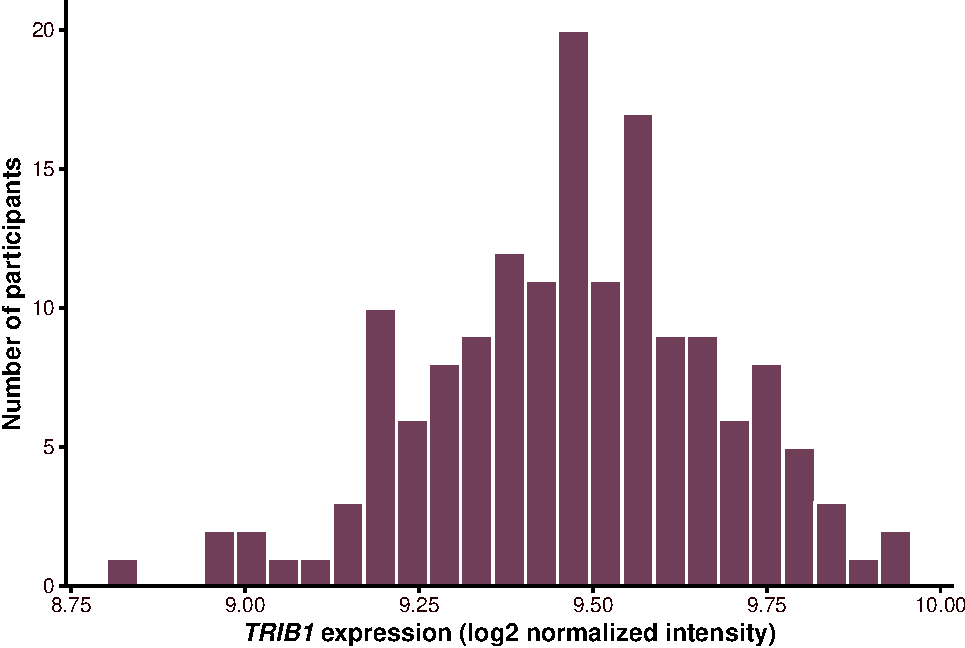
\includegraphics[keepaspectratio,alt={ Expression values from 157 pregnant participants are log2-transformed normalized intensities from the Affymetrix Human Gene 1.0 ST Array, measured in blood collected at 10--19 weeks' gestation.}]{Golden_Kelly_Final_Submission_files/figure-latex/plots-7.pdf}}
\caption{\textbf{Distribution of \textit{TRIB1} expression.} Expression
values from 157 pregnant participants are log2-transformed normalized
intensities from the Affymetrix Human Gene 1.0 ST Array, measured in
blood collected at 10--19 weeks' gestation.}
\end{figure}

\begin{figure}
\centering
\pandocbounded{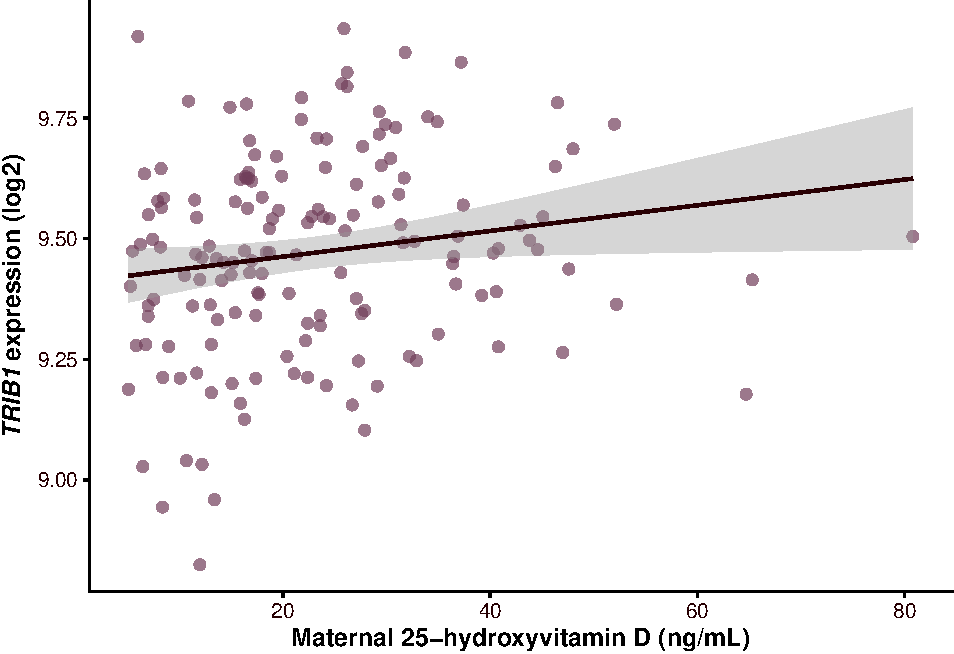
\includegraphics[keepaspectratio,alt={ Each point is one participant (n = 157). The black line is a linear regression fit, and the gray band is its 95\% confidence interval.}]{Golden_Kelly_Final_Submission_files/figure-latex/plots-8.pdf}}
\caption{\textbf{Maternal vitamin D vs. \textit{TRIB1} expression.} Each
point is one participant (n = 157). The black line is a linear
regression fit, and the gray band is its 95\% confidence interval.}
\end{figure}

\begin{figure}
\centering
\pandocbounded{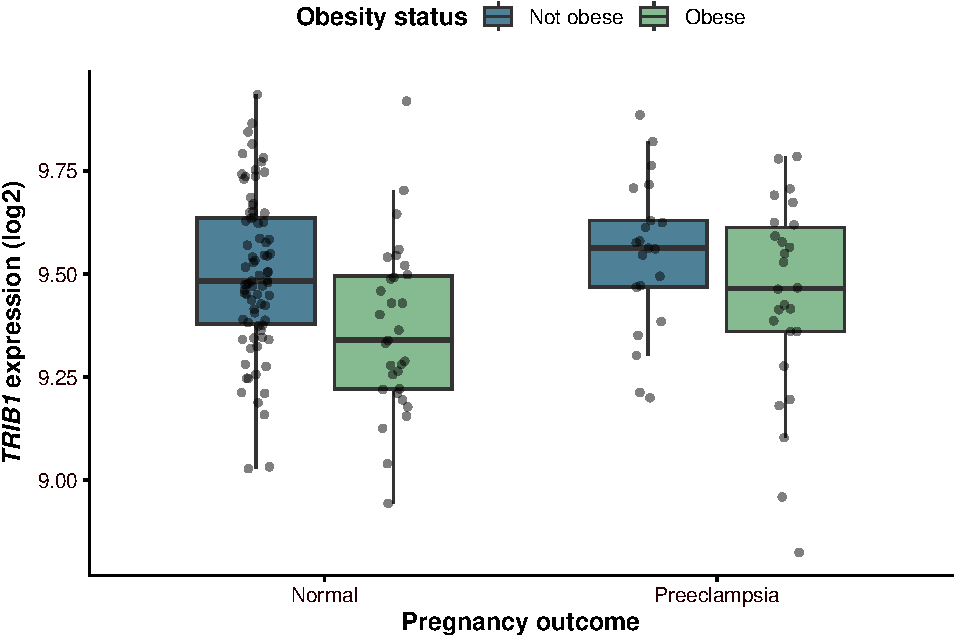
\includegraphics[keepaspectratio,alt={ Obesity was defined as BMI \textbackslash geq 30 kg/m². Boxes show the median and interquartile range, whiskers extend to 1.5 × IQR, and points are individual participants. Group sizes: Normal/not obese n = 79, Normal/obese n = 31, Preeclampsia/not obese n = 21, Preeclampsia/obese n = 26.}]{Golden_Kelly_Final_Submission_files/figure-latex/plots-9.pdf}}
\caption{\textbf{\textit{TRIB1} expression by pregnancy outcome and obesity status.}
Obesity was defined as BMI \(\geq\) 30 kg/m². Boxes show the median and
interquartile range, whiskers extend to 1.5 × IQR, and points are
individual participants. Group sizes: Normal/not obese n = 79,
Normal/obese n = 31, Preeclampsia/not obese n = 21, Preeclampsia/obese n
= 26.}
\end{figure}

\subsection{Table 1 prep (Summary
Statistics)}\label{table-1-prep-summary-statistics}

\begin{Shaded}
\begin{Highlighting}[]
\CommentTok{\# Claude helped figure this code out}

\CommentTok{\# summary statistics for Table 1: maternal age, gestational age at delivery,}
\CommentTok{\# maternal vitamin D (mean and SD), and obesity (n and \%),}
\CommentTok{\# stratified by pregnancy outcome}
\NormalTok{summaryTable1 }\OtherTok{\textless{}{-}}\NormalTok{ covar }\SpecialCharTok{\%\textgreater{}\%} 
  \FunctionTok{group\_by}\NormalTok{(preg\_preeclampsia) }\SpecialCharTok{\%\textgreater{}\%} 
  \FunctionTok{summarise}\NormalTok{(}\AttributeTok{n =} \FunctionTok{n}\NormalTok{(),}
            \AttributeTok{age\_mean     =} \FunctionTok{mean}\NormalTok{(mat\_age\_yrs),}
            \AttributeTok{age\_sd       =} \FunctionTok{sd}\NormalTok{(mat\_age\_yrs),}
            \AttributeTok{gestAge\_mean =} \FunctionTok{mean}\NormalTok{(delivery\_gestAge\_wks),}
            \AttributeTok{gestAge\_sd   =} \FunctionTok{sd}\NormalTok{(delivery\_gestAge\_wks),}
            \AttributeTok{vitD\_mean =} \FunctionTok{mean}\NormalTok{(mat\_vitD),}
            \AttributeTok{vitD\_sd   =} \FunctionTok{sd}\NormalTok{(mat\_vitD),}
            \AttributeTok{obese\_n   =} \FunctionTok{sum}\NormalTok{(obesity }\SpecialCharTok{==} \StringTok{"Obese"}\NormalTok{),}
            \AttributeTok{obese\_pct =} \FunctionTok{mean}\NormalTok{(obesity }\SpecialCharTok{==} \StringTok{"Obese"}\NormalTok{) }\SpecialCharTok{*} \DecValTok{100}\NormalTok{)}

\CommentTok{\# print rounded to one decimal place}
\NormalTok{summaryTable1 }\SpecialCharTok{\%\textgreater{}\%} \FunctionTok{mutate}\NormalTok{(}\FunctionTok{across}\NormalTok{(}\FunctionTok{where}\NormalTok{(is.double), }\SpecialCharTok{\textasciitilde{}} \FunctionTok{round}\NormalTok{(.x, }\DecValTok{1}\NormalTok{)))}
\end{Highlighting}
\end{Shaded}

\begin{verbatim}
## # A tibble: 2 x 10
##   preg_preeclampsia     n age_mean age_sd gestAge_mean gestAge_sd vitD_mean
##   <fct>             <int>    <dbl>  <dbl>        <dbl>      <dbl>     <dbl>
## 1 Normal              110     26.6    5.1         39.3        1        24.4
## 2 Preeclampsia         47     25.8    4.9         37.8        3.5      19.7
## # i 3 more variables: vitD_sd <dbl>, obese_n <int>, obese_pct <dbl>
\end{verbatim}

\subsection{Heatmap}\label{heatmap}

\begin{Shaded}
\begin{Highlighting}[]
\CommentTok{\# Claude helped figure this code out}

\CommentTok{\# 10 genes for the heatmap}
\NormalTok{heatGenes }\OtherTok{\textless{}{-}} \FunctionTok{c}\NormalTok{(}\StringTok{"CXCR2"}\NormalTok{, }\StringTok{"LYN"}\NormalTok{, }\StringTok{"PRKCD"}\NormalTok{, }\StringTok{"AQP9"}\NormalTok{, }\StringTok{"FOSL2"}\NormalTok{,}
               \StringTok{"TRIB1"}\NormalTok{, }\StringTok{"NR0B2"}\NormalTok{, }\StringTok{"ACSL4"}\NormalTok{, }\StringTok{"EPHX2"}\NormalTok{, }\StringTok{"PEX12"}\NormalTok{)}

\NormalTok{heatMat }\OtherTok{\textless{}{-}}\NormalTok{ geneExp }\SpecialCharTok{\%\textgreater{}\%}
  \FunctionTok{filter}\NormalTok{(GENE }\SpecialCharTok{\%in\%}\NormalTok{ heatGenes) }\SpecialCharTok{\%\textgreater{}\%}      \CommentTok{\# keep only the 10 genes}
  \FunctionTok{select}\NormalTok{(}\SpecialCharTok{{-}}\NormalTok{PROBEID) }\SpecialCharTok{\%\textgreater{}\%}                 \CommentTok{\# remove the probe ID column}
  \FunctionTok{column\_to\_rownames}\NormalTok{(}\StringTok{"GENE"}\NormalTok{) }\SpecialCharTok{\%\textgreater{}\%}       \CommentTok{\# gene names become row names}
  \FunctionTok{as.matrix}\NormalTok{()                          }\CommentTok{\# convert to a numeric matrix}

\FunctionTok{dim}\NormalTok{(heatMat) }\CommentTok{\# expect 10 157}
\end{Highlighting}
\end{Shaded}

\begin{verbatim}
## [1]  10 157
\end{verbatim}

\begin{Shaded}
\begin{Highlighting}[]
\CommentTok{\# tracking{-}bar annotations: one row per participant, matched to heatMat columns}
\NormalTok{annotCol }\OtherTok{\textless{}{-}}\NormalTok{ covar }\SpecialCharTok{\%\textgreater{}\%}
  \FunctionTok{select}\NormalTok{(geoID, preg\_preeclampsia, obesity) }\SpecialCharTok{\%\textgreater{}\%}
  \FunctionTok{rename}\NormalTok{(}\AttributeTok{Preeclampsia =}\NormalTok{ preg\_preeclampsia,   }\CommentTok{\# nicer names for the legend}
         \AttributeTok{Obesity =}\NormalTok{ obesity) }\SpecialCharTok{\%\textgreater{}\%}
  \FunctionTok{column\_to\_rownames}\NormalTok{(}\StringTok{"geoID"}\NormalTok{)}

\CommentTok{\# put the rows in the same order as the heatmap columns}
\NormalTok{annotCol }\OtherTok{\textless{}{-}}\NormalTok{ annotCol[}\FunctionTok{colnames}\NormalTok{(heatMat), ]}

\CommentTok{\# check the order matches exactly}
\FunctionTok{all}\NormalTok{(}\FunctionTok{rownames}\NormalTok{(annotCol) }\SpecialCharTok{==} \FunctionTok{colnames}\NormalTok{(heatMat)) }\CommentTok{\# expect TRUE}
\end{Highlighting}
\end{Shaded}

\begin{verbatim}
## [1] TRUE
\end{verbatim}

\begin{Shaded}
\begin{Highlighting}[]
\CommentTok{\# colors for the tracking bars (reuse obesity colors so all figures match)}
\NormalTok{annotColors }\OtherTok{\textless{}{-}} \FunctionTok{list}\NormalTok{(}
  \AttributeTok{Preeclampsia =} \FunctionTok{c}\NormalTok{(}\StringTok{"Normal"} \OtherTok{=} \StringTok{"\#D9D9D9"}\NormalTok{, }\StringTok{"Preeclampsia"} \OtherTok{=} \StringTok{"\#713E5A"}\NormalTok{),}
  \AttributeTok{Obesity      =}\NormalTok{ obesityColors}
\NormalTok{)}

\CommentTok{\# color scale for expression: purple (low) {-}\textgreater{} white (average) {-}\textgreater{} orange (high)}
\NormalTok{heatColors }\OtherTok{\textless{}{-}} \FunctionTok{colorRampPalette}\NormalTok{(}\FunctionTok{c}\NormalTok{(}\StringTok{"\#5E3C99"}\NormalTok{, }\StringTok{"white"}\NormalTok{, }\StringTok{"\#E66101"}\NormalTok{))(}\DecValTok{100}\NormalTok{)}

\FunctionTok{pheatmap}\NormalTok{(heatMat,}
         \AttributeTok{scale =} \StringTok{"row"}\NormalTok{,               }\CommentTok{\# z{-}score each gene across participants}
         \AttributeTok{color =}\NormalTok{ heatColors,}
         \AttributeTok{clustering\_distance\_rows =} \StringTok{"euclidean"}\NormalTok{,}
         \AttributeTok{clustering\_distance\_cols =} \StringTok{"euclidean"}\NormalTok{,}
         \AttributeTok{clustering\_method =} \StringTok{"complete"}\NormalTok{,}
         \AttributeTok{annotation\_col =}\NormalTok{ annotCol, }
         \AttributeTok{annotation\_colors =}\NormalTok{ annotColors,}
         \AttributeTok{breaks =} \FunctionTok{seq}\NormalTok{(}\SpecialCharTok{{-}}\DecValTok{3}\NormalTok{, }\DecValTok{3}\NormalTok{, }\AttributeTok{length.out =} \DecValTok{101}\NormalTok{),}
         \AttributeTok{show\_colnames =} \ConstantTok{FALSE}\NormalTok{,        }\CommentTok{\# hide participant IDs}
         \AttributeTok{labels\_row =} \FunctionTok{as.expression}\NormalTok{(}\FunctionTok{lapply}\NormalTok{(}\FunctionTok{rownames}\NormalTok{(heatMat),}
                                           \ControlFlowTok{function}\NormalTok{(x) }\FunctionTok{bquote}\NormalTok{(}\FunctionTok{italic}\NormalTok{(.(x))))),}
         \AttributeTok{border\_color =} \ConstantTok{NA}\NormalTok{)}
\end{Highlighting}
\end{Shaded}

\begin{figure}
\centering
\pandocbounded{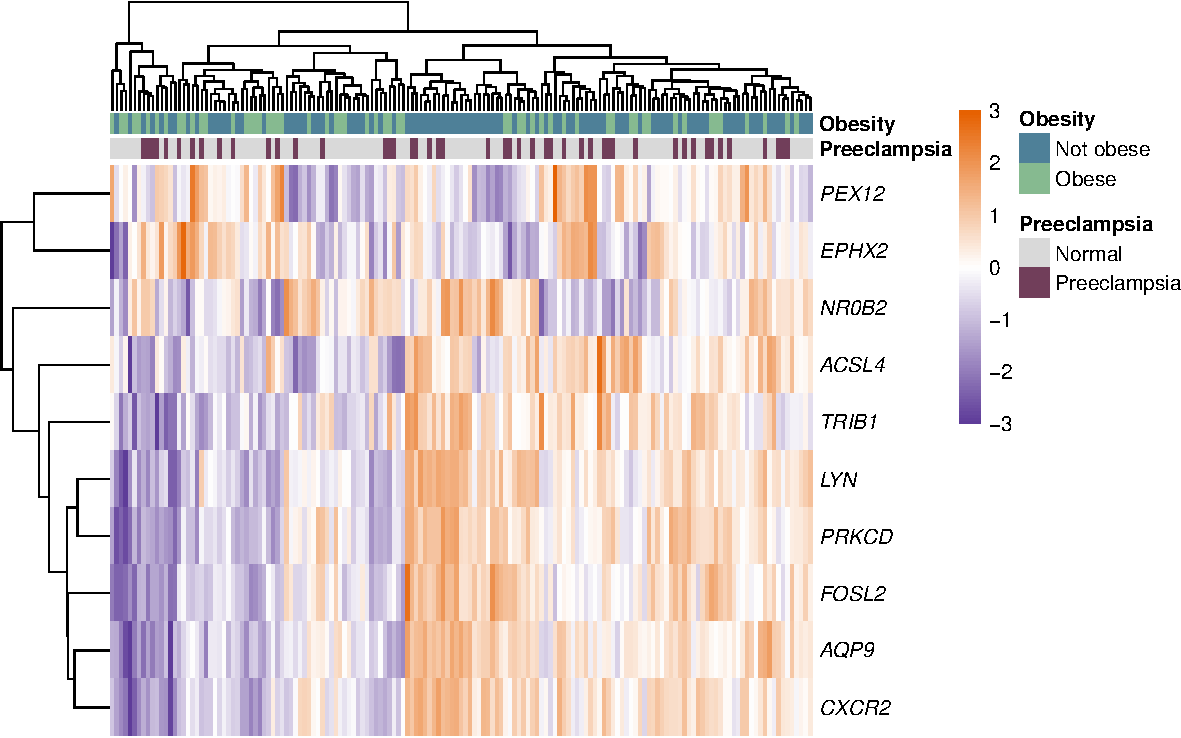
\includegraphics[keepaspectratio,alt={ Colors show gene expression z-scores (each gene scaled across participants; values beyond ±3 shown at the darkest color). Genes and participants were clustered by hierarchical clustering (Euclidean distance, complete linkage). Tracking bars show pregnancy outcome and obesity status (BMI \textbackslash geq 30 kg/m\^{}2).}]{Golden_Kelly_Final_Submission_files/figure-latex/heatmap-1.pdf}}
\caption{\textbf{Expression of ten inflammation- and metabolism-related genes across 157 participants.}
Colors show gene expression z-scores (each gene scaled across
participants; values beyond ±3 shown at the darkest color). Genes and
participants were clustered by hierarchical clustering (Euclidean
distance, complete linkage). Tracking bars show pregnancy outcome and
obesity status (BMI \(\geq\) 30 kg/m\(^2\)).}
\end{figure}

\subsection{Forest plot}\label{forest-plot}

\begin{Shaded}
\begin{Highlighting}[]
\CommentTok{\# Claude helped figure this code out}
\CommentTok{\# vitamin D per 10 ng/mL so regression estimates are easier to read}
\NormalTok{datAll }\OtherTok{\textless{}{-}}\NormalTok{ datAll }\SpecialCharTok{\%\textgreater{}\%} \FunctionTok{mutate}\NormalTok{(}\AttributeTok{vitD10 =}\NormalTok{ mat\_vitD }\SpecialCharTok{/} \DecValTok{10}\NormalTok{)}

\CommentTok{\# fit unadjusted and obesity{-}adjusted models for each gene,}
\CommentTok{\# keeping the vitamin D estimate and 95\% CI}
\NormalTok{forestDat }\OtherTok{\textless{}{-}} \FunctionTok{data.frame}\NormalTok{()   }\CommentTok{\# start with an empty data frame}

\ControlFlowTok{for}\NormalTok{ (g }\ControlFlowTok{in}\NormalTok{ heatGenes) \{}
\NormalTok{  geneData }\OtherTok{\textless{}{-}}\NormalTok{ datAll }\SpecialCharTok{\%\textgreater{}\%} \FunctionTok{filter}\NormalTok{(GENE }\SpecialCharTok{==}\NormalTok{ g)}

\NormalTok{  m1 }\OtherTok{\textless{}{-}} \FunctionTok{lm}\NormalTok{(expression }\SpecialCharTok{\textasciitilde{}}\NormalTok{ vitD10, }\AttributeTok{data =}\NormalTok{ geneData)           }\CommentTok{\# unadjusted}
\NormalTok{  m2 }\OtherTok{\textless{}{-}} \FunctionTok{lm}\NormalTok{(expression }\SpecialCharTok{\textasciitilde{}}\NormalTok{ vitD10 }\SpecialCharTok{+}\NormalTok{ obesity, }\AttributeTok{data =}\NormalTok{ geneData) }\CommentTok{\# adjusted for obesity}

\NormalTok{  forestDat }\OtherTok{\textless{}{-}} \FunctionTok{rbind}\NormalTok{(forestDat,}
    \FunctionTok{data.frame}\NormalTok{(}\AttributeTok{gene =}\NormalTok{ g, }\AttributeTok{model =} \StringTok{"Unadjusted"}\NormalTok{,}
               \AttributeTok{estimate =} \FunctionTok{coef}\NormalTok{(m1)[}\StringTok{"vitD10"}\NormalTok{],}
               \AttributeTok{lower =} \FunctionTok{confint}\NormalTok{(m1)[}\StringTok{"vitD10"}\NormalTok{, }\DecValTok{1}\NormalTok{],}
               \AttributeTok{upper =} \FunctionTok{confint}\NormalTok{(m1)[}\StringTok{"vitD10"}\NormalTok{, }\DecValTok{2}\NormalTok{]),}
    \FunctionTok{data.frame}\NormalTok{(}\AttributeTok{gene =}\NormalTok{ g, }\AttributeTok{model =} \StringTok{"Adjusted for obesity"}\NormalTok{,}
               \AttributeTok{estimate =} \FunctionTok{coef}\NormalTok{(m2)[}\StringTok{"vitD10"}\NormalTok{],}
               \AttributeTok{lower =} \FunctionTok{confint}\NormalTok{(m2)[}\StringTok{"vitD10"}\NormalTok{, }\DecValTok{1}\NormalTok{],}
               \AttributeTok{upper =} \FunctionTok{confint}\NormalTok{(m2)[}\StringTok{"vitD10"}\NormalTok{, }\DecValTok{2}\NormalTok{]))}
\NormalTok{\}}

\FunctionTok{nrow}\NormalTok{(forestDat)   }\CommentTok{\# expect 20}
\end{Highlighting}
\end{Shaded}

\begin{verbatim}
## [1] 20
\end{verbatim}

\begin{Shaded}
\begin{Highlighting}[]
\CommentTok{\# order genes top to bottom as in heatGenes, and fix the model order}
\NormalTok{forestDat }\OtherTok{\textless{}{-}}\NormalTok{ forestDat }\SpecialCharTok{\%\textgreater{}\%}
  \FunctionTok{mutate}\NormalTok{(}\AttributeTok{gene  =} \FunctionTok{factor}\NormalTok{(gene, }\AttributeTok{levels =} \FunctionTok{rev}\NormalTok{(heatGenes)),}
         \AttributeTok{model =} \FunctionTok{factor}\NormalTok{(model, }\AttributeTok{levels =} \FunctionTok{c}\NormalTok{(}\StringTok{"Adjusted for obesity"}\NormalTok{, }\StringTok{"Unadjusted"}\NormalTok{)))}

\NormalTok{forestPlot }\OtherTok{\textless{}{-}} \FunctionTok{ggplot}\NormalTok{(forestDat, }\FunctionTok{aes}\NormalTok{(}\AttributeTok{x =}\NormalTok{ gene, }\AttributeTok{y =}\NormalTok{ estimate, }\AttributeTok{color =}\NormalTok{ model)) }\SpecialCharTok{+}
  \CommentTok{\#line of no association}
  \FunctionTok{geom\_hline}\NormalTok{(}\AttributeTok{yintercept =} \DecValTok{0}\NormalTok{, }\AttributeTok{linetype =} \StringTok{"dashed"}\NormalTok{, }\AttributeTok{color =} \StringTok{"\#280003"}\NormalTok{) }\SpecialCharTok{+}
  \FunctionTok{geom\_pointrange}\NormalTok{(}\FunctionTok{aes}\NormalTok{(}\AttributeTok{ymin =}\NormalTok{ lower, }\AttributeTok{ymax =}\NormalTok{ upper),}
                  \CommentTok{\# dot= estimate, line = 95\% CI}
                  \AttributeTok{position =} \FunctionTok{position\_dodge}\NormalTok{(}\AttributeTok{width =} \FloatTok{0.4}\NormalTok{)) }\SpecialCharTok{+}  
  \FunctionTok{coord\_flip}\NormalTok{() }\SpecialCharTok{+}      \CommentTok{\# genes on the side}
  \FunctionTok{scale\_color\_manual}\NormalTok{(}\AttributeTok{values =} \FunctionTok{c}\NormalTok{(}\StringTok{"Unadjusted"} \OtherTok{=} \StringTok{"\#713E5A"}\NormalTok{,}
                                \StringTok{"Adjusted for obesity"} \OtherTok{=} \StringTok{"gray50"}\NormalTok{),}
                     \AttributeTok{breaks =} \FunctionTok{c}\NormalTok{(}\StringTok{"Unadjusted"}\NormalTok{, }\StringTok{"Adjusted for obesity"}\NormalTok{),}
                     \AttributeTok{name =} \ConstantTok{NULL}\NormalTok{) }\SpecialCharTok{+}
  \FunctionTok{scale\_y\_continuous}\NormalTok{(}\AttributeTok{breaks =} \FunctionTok{seq}\NormalTok{(}\SpecialCharTok{{-}}\FloatTok{0.04}\NormalTok{, }\FloatTok{0.12}\NormalTok{, }\AttributeTok{by =} \FloatTok{0.02}\NormalTok{)) }\SpecialCharTok{+}
  \FunctionTok{labs}\NormalTok{(}\AttributeTok{x =} \ConstantTok{NULL}\NormalTok{,}
       \AttributeTok{y =} \StringTok{"Change in expression (log2) per 10 ng/mL vitamin D (95\% CI)"}\NormalTok{) }\SpecialCharTok{+}
  
\NormalTok{  theme\_pub }\SpecialCharTok{+}
  \FunctionTok{theme}\NormalTok{(}\AttributeTok{axis.text.y =} \FunctionTok{element\_text}\NormalTok{(}\AttributeTok{face =} \StringTok{"italic"}\NormalTok{))}

\NormalTok{forestPlot}
\end{Highlighting}
\end{Shaded}

\begin{figure}
\centering
\pandocbounded{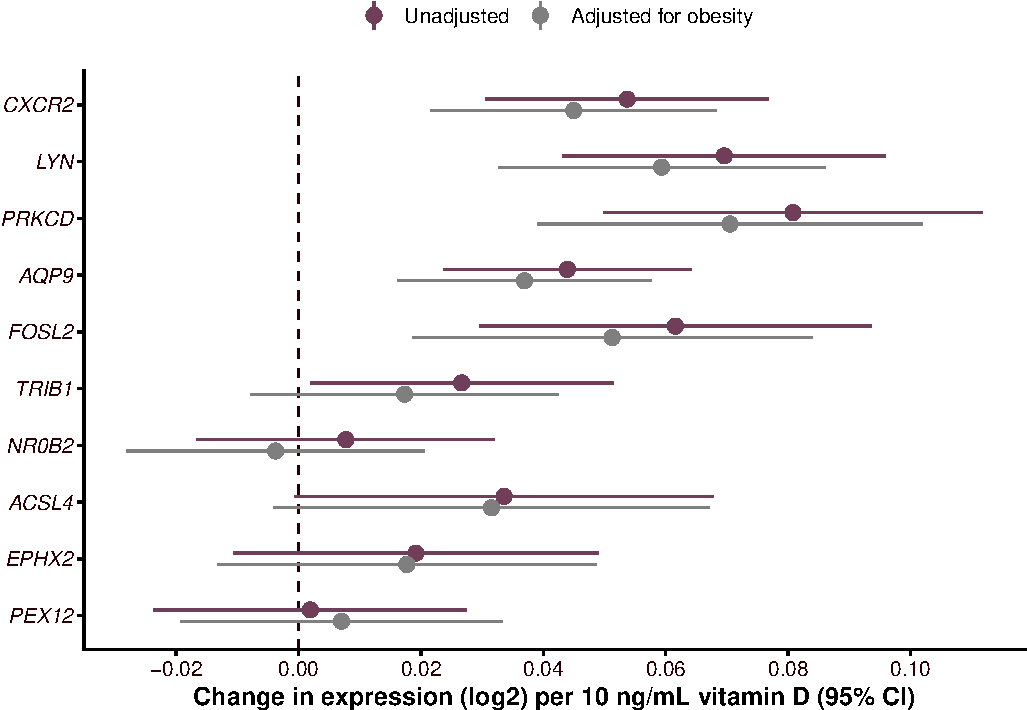
\includegraphics[keepaspectratio,alt={ Points show the estimated change in log2 expression per 10 ng/mL increase in 25-hydroxyvitamin D from linear regression; lines show 95\% confidence intervals. Purple: unadjusted model; gray: model adjusted for obesity (BMI \textbackslash geq 30 kg/m\^{}2). The dashed line marks no association. n = 157.}]{Golden_Kelly_Final_Submission_files/figure-latex/forest-1.pdf}}
\caption{\textbf{Association between maternal vitamin D and expression of ten inflammation- and metabolism-related genes, before and after adjustment for obesity.}
Points show the estimated change in log2 expression per 10 ng/mL
increase in 25-hydroxyvitamin D from linear regression; lines show 95\%
confidence intervals. Purple: unadjusted model; gray: model adjusted for
obesity (BMI \(\geq\) 30 kg/m\(^2\)). The dashed line marks no
association. n = 157.}
\end{figure}

\begin{Shaded}
\begin{Highlighting}[]
\FunctionTok{ggsave}\NormalTok{(}\StringTok{"forest\_plot.pdf"}\NormalTok{, forestPlot, }\AttributeTok{width =} \DecValTok{7}\NormalTok{, }\AttributeTok{height =} \DecValTok{5}\NormalTok{)}
\end{Highlighting}
\end{Shaded}

\subsection{Software Version}\label{software-version}

\begin{Shaded}
\begin{Highlighting}[]
\NormalTok{R.version.string}
\end{Highlighting}
\end{Shaded}

\begin{verbatim}
## [1] "R version 4.6.1 (2026-06-24)"
\end{verbatim}

\begin{Shaded}
\begin{Highlighting}[]
\FunctionTok{packageVersion}\NormalTok{(}\StringTok{"tidyverse"}\NormalTok{); }\FunctionTok{packageVersion}\NormalTok{(}\StringTok{"ggplot2"}\NormalTok{); }\FunctionTok{packageVersion}\NormalTok{(}\StringTok{"pheatmap"}\NormalTok{)}
\end{Highlighting}
\end{Shaded}

\begin{verbatim}
## [1] '2.0.0'
\end{verbatim}

\begin{verbatim}
## [1] '4.0.3'
\end{verbatim}

\begin{verbatim}
## [1] '1.0.13'
\end{verbatim}

\end{document}
